\documentclass[notitlepage]{article}

\usepackage{titling}

\pretitle{\begin{center}\huge\bfseries}
\posttitle{\par\end{center}\vskip 0.5em}
\preauthor{\begin{center}\Large}
\postauthor{\end{center}}
\predate{\par\large\centering}
\postdate{\par}

\usepackage{graphicx}
\usepackage{mathpartir}
\usepackage{amssymb}
\usepackage{xspace}
\usepackage{stmaryrd}
\usepackage{listings}
\usepackage{float}
\usepackage{rotating}
\usepackage[backend=bibtex, sorting=none, maxbibnames=99]{biblatex}
\usepackage{parskip}
\usepackage{pdfpages}
\usepackage{hyperref}
\usepackage{xspace}
\usepackage{geometry}
\usepackage{pgfplots}
\pgfplotsset{width=7cm,compat=1.8}
\usepackage{pgfplotstable}
\renewcommand*{\familydefault}{\sfdefault}

\geometry{
	paper=a4paper, % Change to letterpaper for US letter
	margin=3cm
}

\newcommand{\lang}{\textsc{Effy}\xspace}
\newcommand{\eff}{\textsc{Eff}\xspace}
\newcommand{\ocaml}{\textsc{OCaml}\xspace}

% Meta-syntax
\newcommand{\bnfis}{\mathrel{\;{:}{:}\!=}\;}
\newcommand{\bnfor}{\mathrel{\;|\;}}
\newcommand{\defeq}{\mathrel{\;\stackrel{\text{def}}{=}\;}}
\newcommand{\set}[1]{\{ #1 \}}

% General syntactic constructs
\newcommand{\kord}[1]{\mathtt{#1}}
\newcommand{\kop}[1]{\;\mathtt{#1}\;}
\newcommand{\kpre}[1]{\mathtt{#1}\;}
\newcommand{\kpost}[1]{\;\mathtt{#1}}

% Types
\newcommand{\type}[1]{\mathtt{#1}}
\newcommand{\boolty}{\type{bool}}
\newcommand{\intty}{\type{int}}
\newcommand{\hto}{\Rightarrow}
\newcommand{\C}{\underline{C}}
\newcommand{\D}{\underline{D}}
\newcommand{\dirt}{\Delta}
\newcommand{\sig}{\Sigma}

% Expressions and computations
\newcommand{\call}[3]{{{#1}\,{#2}\,{#3}}}
\newcommand{\case}{\mathop{\text{\texttt{|}}}}
\newcommand{\cont}[2]{(#1.\,#2)}
\newcommand{\const}{\kord{k}}
\newcommand{\fls}{\kord{false}}
\newcommand{\fun}[1]{\kpre{fun} #1 \mapsto}
\newcommand{\handler}[1]{\{ #1 \}}
\newcommand{\conditional}[3]{\kpre{if} #1 \kop{then} #2 \kop{else} #3}
\newcommand{\letin}[1]{\kpre{let} #1 \kop{in}}
\newcommand{\doin}[1]{\kpre{do} #1 \kop{ ; }}
\newcommand{\letrecin}[1]{\kpre{let} \kpre{rec} #1 \kop{in}}
\newcommand{\op}{\kord{Op}}
\newcommand{\ops}{\mathcal{O}}
\newcommand{\ocs}{\mathit{ocs}}
\newcommand{\ocsnil}{\kord{nil}}
\newcommand{\tru}{\kord{true}}
\newcommand{\ret}{\kpre{return}}
\newcommand{\withhandle}[2]{\kpre{handle} #2 \kop{with} #1}
\newcommand{\pure}[1]{\kord{pure } #1  }
\newcommand{\longcases}{\call{\op_1}{x}{k} \mapsto c_{\op_1}, \ldots, \call{\op_n}{x}{k} \mapsto c_{\op_n}}
\newcommand{\shortcases}{[\call{\op}{x}{k} \mapsto c_\op]_{\op \in \ops}}
\newcommand{\longhand}[1][\ret x \mapsto c_r]{\handler{#1, \longcases}}
\newcommand{\shorthand}[1][\ret x \mapsto c_r]{\handler{#1, \shortcases}}

% Type-checking
\newcommand{\ctx}{\Gamma}
\newcommand{\ent}{\vdash}
\newcommand{\T}{\mathrel{:}}
\newcommand{\E}{\mathrel{!}}
\newcommand{\covers}{\mathrel{/}}
\renewcommand{\le}{\leqslant}

% Operational semantics
\newcommand{\eval}{\Downarrow}
\newcommand{\hs}{\mathcal{H}}
\newcommand{\nil}{\emptyset}
\newcommand{\cons}{\mathbin{::}}
\newcommand{\hseval}[1][\hs]{\Downarrow_{#1}}
\newcommand{\getval}[1]{{#1}_{\kord{val}}}
\newcommand{\getop}[1]{{#1}_{\kord{op}}}

%functions

\newcommand{\inlinable}[3]{\textit{inlinable(}#1, #2 ,#3 \textit{)}}


\newcommand{\queens}[1]{\textit{#1-Queens}\xspace}
\newcommand{\loops}{\textit{Loop}}

\newcommand{\todo}[1]{\textcolor{red}{\textsc{TODO:} #1}}
\newcommand{\rules}[1]{\textcolor{green}{\textsc{Rule:} #1}}
\newcommand{\feedback}[2]{\textcolor{blue}{\textsc{#1}:#2}}

\lstset{%
language=Caml,
moredelim=*[is][\itshape]{/@}{@/},
numbers=none,mathescape=true,showstringspaces=false,
morekeywords={handle,handler,with,val},
keywordstyle=\bfseries,
xleftmargin=1em,basicstyle=\ttfamily\small}
\lstnewenvironment{source}{\lstset{
basicstyle=\ttfamily\small,
% Uncomment to enable bold keywords in source environments
% keywordstyle=\bfseries
}}{}
\newcommand{\effcode}[1]{\textcolor{magenta}{\lstinline{#1}}}
\newcommand{\ocamlcode}[1]{\textcolor{teal}{\lstinline{#1}}}
\lstnewenvironment{efflisting}{\lstset{breaklines=true,
postbreak=\raisebox{0ex}[0ex][0ex]{\ensuremath{\color{red}\hookrightarrow\space}},basicstyle=\ttfamily\small\color{magenta}}}{}
\lstnewenvironment{ocamllisting}{\lstset{breaklines=true,
postbreak=\raisebox{0ex}[0ex][0ex]{\ensuremath{\color{red}\hookrightarrow\space}},basicstyle=\ttfamily\small\color{teal}}}{}
\lstnewenvironment{linkslisting}{\lstset{breaklines=true,
postbreak=\raisebox{0ex}[0ex][0ex]{\ensuremath{\color{red}\hookrightarrow\space}},basicstyle=\ttfamily\small\color{blue}}}{}

\bibliography{evaluation.bib} 

\title{\vspace{-2cm}Honoursprogramme: Research track, option A (9 ECTS) \\\mbox{}\\ {Efficient Compilation of Algebraic Effects and Handlers in Eff}}
\author{Student: Axel Faes\\{ Promotor: Prof. dr. ir. Tom Schrijvers}\\{Daily supervisors:  Prof. dr. ir. Tom Schrijvers \&\\ Amr Hany Shehata Saleh}\\\mbox{}\\{Master in de ingenieurswetenschappen: \\computerwetenschappen}\\{Specialisatie: Artificial Intelligence}\\{Fase 1}}
\date{September 2016 - March 2017}

\begin{document}

\maketitle

\tableofcontents

\section{Description}
\subsection{Introduction}
My honoursproject was part of the C1 project \textit{Algebraic Effect Handlers: Harnessing the Fundamental Powers of Effects} \cite{project}. During my honoursproject I had to work on the \eff programming language. More specifically, I had to create optimizations within the compiler in order to optimize away effect handlers. More specifically, my honoursproject can be broken down in the following steps:
\begin{enumerate}
\item Literature study of Eff and existing optimizations 
\item Designing and implement new optimizations
\item evaluation: Eff versus OCaml
\item evaluation: Eff versus Other Systems
\end{enumerate}
As we are working with both \ocaml and \eff, whose syntax closely follows \ocaml, colors are used to distinguish between \ocamlcode{OCaml code} and \effcode{Eff code}. A paper was written towards the end of my honoursproject. The paper has been submitted and is currently in review. The abstract of the paper reads as follows: \cite{own}
\begin{quotation}
\noindent The popularity of algebraic effect handlers as a programming language feature for user-defined computational effects is steadily growing. Yet, even though efficient runtime representations have already been studied, most handler-based programs are still much slower than hand-written code.\\
\\
In this paper we show that the performance gap can be drastically narrowed (in some cases even closed) by means of type-and-effect directed optimising compilation. Our approach consists of two stages. Firstly, we combine elementary source-to-source transformations with judicious function specialisation in order to aggressively reduce handler applications. Secondly, we show how to elaborate the source language into a handler-less target language in a way that incurs no overhead for pure computations.\\
\\
This work comes with a practical implementation: an optimizing compiler from \eff, an ML style language with algebraic effect handlers, to \ocaml. Experimental evaluation with this implementation demonstrates that in a number of benchmarks, our approach eliminates much of the overhead of handlers and yields competitive performance with hand-written \ocaml code.
\end{quotation}

\subsection{Overview of Eff}
\eff is a ML style functional programming language that uses algebraic effect handlers \cite{eff}. These handlers can be used to easily implement I/O, non-determinism or backtracking. \eff compiles down to \ocaml code. The naive translation for effect handlers is very slow compared to a native implementation in OCaml or an implementation in Multicore \ocaml \cite{KCeff}. Below is (part of) the naive translation of the N-queens program. \label{queenscomp}
\begin{ocamllisting}
type (_, _) effect += Effect_decide : (unit, bool) effect
type (_, _) effect += Effect_fail : (unit, 'empty) effect

let decide x = call Effect_decide () value
let fail () = call Effect_fail () (fun _ -> assert false)

let choose_all = handler {
  value_clause = (fun x -> [x]);
  effect_clauses = fun (type a) (type b) (eff : (a, b) effect) -> (
    match eff with
    | Effect_decide -> fun _ k ->
        (k true @ k false)
    | Effect_fail -> fun _ _ ->
        []
    :
    a -> (b -> _) -> _
  )
}

let queens number_of_queens =
  let rec place (x, qs) =
    if x > number_of_queens then value qs else
      choose (available (number_of_queens, x, qs)) >>
      fun y -> (place (x + 1, (x, y) :: qs))
  in
  place (1, [])
  
let queens_all number_of_queens =
  choose_all (queens number_of_queens)
\end{ocamllisting}
The native (hand-written) code looks as follows: \label{queensnative}
\begin{ocamllisting}
let queens_all number_of_queens =
  let rec place (x, qs) =
    if x > number_of_queens then [qs] else
      let rec choose = function
        | [] -> []
        | y :: ys ->
            place ((x + 1), ((x, y) :: qs)) @ choose ys
      in
      choose (available (number_of_queens, x, qs))
  in
  place (1, [])
\end{ocamllisting}
The \eff code looks as follows: \label{queenseff}
\begin{efflisting}
effect Decide : unit -> bool
effect Fail : unit -> empty

let choose_all = handler
  | val x -> [x]
  | #Decide _ k -> k true @ k false
  | #Fail _ _ -> []
  
let queens number_of_queens =
  let rec place (x, qs) =
    if x > number_of_queens then qs else
      let y = choose (available (number_of_queens, x, qs)) in
      place ((x + 1), ((x, y) :: qs))
  in
  place (1, [])

let queens_all number_of_queens =
  with choose_all handle queens number_of_queens
\end{efflisting}
The naive compilation is ~100 times slower compared to the native code. Through the optimised compilation, the produced code becomes as fast the the native code. An advantage to the \eff code is that we can make the queens function perform differently depending on how the effects are implemented. This compared to the native version which is different for each implementation. It can be seen that in the naive translation, there is still a seperate datastructure for the effect handler. This means that each time an effect occurs, it has to go through the effect handler. 

\subsection{Literature study}
The honoursproject was started in September 2016. In the beginning of the honoursproject, I had to get a good grasp of what I could contribute to the \eff language. I got familiar with algebraic effects and handlers aswell as the Eff programming language (and its compiler). My main resources were several publications on algebraic effect handlers, \eff and \eff's effects system \cite{introduction} \cite{effectsystem} \cite{inferring} \cite{handling} \cite{programming} \cite{monads}. I also had to learn how to work in \ocaml. This took me a couple weeks. The main issue that I encountered was completely understanding which optimization were already implemented and what they exactly did. Another issue I encountered was being able to work with the type-\&-effect system of \eff. 

\subsection{Optimizations}
Eventually, by the end of October, I had resolved these issues and was able to contribute to the project. During the following weeks I implemented several optimizations. The first optimization I implemented was an optimization that would remove a handler if the computation that the handler is handling was pure. This means that \effcode{with h handle (c)} would be optimized to \effcode{c}. A pure computation is a computation that does not and can not contain effects. \\
\\
Another optimization that I did was the situation where \effcode{with h handle (c1 >> c2)} occurs and \effcode{c1} is pure for handler \effcode{h}. This can be optimized to \effcode{c1 >> (with h handle (c2))}. \\
\\
It was also possible to consider to opposite situation, the scenario where \effcode{c2} is pure for handler \effcode{h}. This optimization becomes a bit more tricky. The code \effcode{with h handle (c1 >> c2)} can be rewritten as \effcode{with h' handle (c1)} with \effcode{h'} a rewritten handler. The \effcode{h'} handler contains the same effect clauses, but has a different value clause compared to the \effcode{h} handler. The value clause can be rewritten as \effcode{c2 >> h.value_clause}. \\
\\
Also the situation where neither \effcode{c1} nor \effcode{c2} are pure for handler \effcode{h}. It still is interesting to split up the handler. Doing that might cause the compiler to see different optimization that could be done. This optimization is similar to the previous one, except that the value clause is rewritten differently. The value clause is rewritten as \effcode{with h handle c1}. \\
\\
The final optimization that I made was the optimization of \effcode{with h handle (let rec defs = ... in c)}. This can be rewritten as \effcode{let rec defs = ... in (with h handle c)}. \\
\\
The code for these optimizations can be found in Appendix~\ref{code}. The formal rules for the rewriting rules are listed in Figure~\ref{fig:rewriterules}. These rules form the minimal set of rewriting rules. During the time that the optimizations were made, I also worked on general bug fixing. The main work for the optimizations was done by the end of December. At this time, I started working on the benchmarks.
\begin{figure}[H]
\begin{center}
\framebox{
\begin{minipage}{0.95\columnwidth}
\textbf{Simplification}\\
\begin{mathpar}
  \inferrule[App-Fun]{
% \textit{inlinable}(x, e ,c)
  }{
    (\fun{x} c) \, v \leadsto c [v/x]
  }

  \inferrule[Do-Ret]{
% \textit{inlinable}(x, e ,c)
  }{
    \doin{x \leftarrow \ret v} c \leadsto c [v / x]
  }


  \inferrule[Do-Op]{
  }{
    \doin{x \leftarrow (\doin{ y \leftarrow \op \,v } c_1 )} c_2 
    \quad\leadsto\quad
    \doin{y \leftarrow \op \,v} (\doin{x \leftarrow c_1} c_2)
  }

\end{mathpar}
\textbf{Handler Reduction}
\begin{mathpar}
  \inferrule[With-LetRec]{
  }{
    \withhandle{v}{(\letrecin{f \, x = c_1} c_2)} \leadsto
    \letrecin{f \, x = c_1} (\withhandle{v}{c_2}) 
  }

  \inferrule[With-Ret]{
    h = \shorthand
  }{
    \withhandle{h}{(\ret v)} \leadsto c_r[v/x]
  }

  \inferrule[With-Handled-Op]{
  \begin{array}{lr}
    h = \shorthand
  \end{array}
  }{
    \withhandle{h}{(\op \, v)} \leadsto
    c_\op[v / x, (\fun{x} c_r) / k]
  }

  \inferrule[With-Pure]{
     h = \shorthand \\
     \Gamma \vdash c : A \E \dirt \\
     \dirt \cap \ops = \emptyset
  }{
    \withhandle{h}{c} \leadsto \doin{x \leftarrow c} c_r
  }

  \inferrule[With-Do]{
    h = \shorthand \\
    h' = \shorthand[\ret y \mapsto (\withhandle{h}{c_2})]
  }
    {
    \withhandle{h}{(\doin{y \leftarrow c_1} c_2)} \leadsto
    \withhandle{h'}{c_1}
  }
\end{mathpar}
\end{minipage}
}
\end{center}
\caption{Term Rewriting Rules \cite{own}}\label{fig:rewriterules}
\end{figure}

\subsection{Evaluation: Eff versus OCaml}
For the evaluation of the optimizations, multiple benchmarks were used. Some simple loop benchmarks were used and a N-queens benchmark. There was a need for some more complex benchmarks to test the optimizations in bigger example programs. For this, an interpreter and a parser were chosen. Four different loop benchmarks were implemented. A pure loop program, to test the conversion from pure \eff code to \ocaml.  A loop program which has an effect \effcode{Fail} that is called when the loop is started with a negative amount of iterations. The final two loop benchmarks are similar to eachother, one increments a value, the other keeps state using a \effcode{Get} and \effcode{Put} effect.\\
\\
The interpreter is a program that takes an AST as input and returns a result. The interpreter is based on an algorithm given by an existing published paper, Monad Transformers and Modular Interpreters,  to make sure that a standard implementation was used \cite{interpreter}. The published paper showed that build a fully modular interpreter based on monad transformers. Not just an \eff version had to be made, but also an version in \ocaml, to be able to compare the performance. \\
\\
The parser is also based on an example from another published paper, Effect Handlers in Scope, which contained several examples concerning grammers and parsers, implemented in Haskell \cite{scope}. Similar to the interpreter, not just an \eff version had to be made. Also an \ocaml version was made to be able to compare the performance. \\
\\
The N-queens benchmarks is implemented in two different versions. The first version, \effcode{queens\_all}, calculates all possible solutions to a given N-queens problem. The other version, \effcode{queens\_one},  only computes the first solution found to a given N-queens problem. The \effcode{queens\_one} version has two different implementations. The first implementation uses an \effcode{Option} datatype, the other implementation uses a \textit{continuation passing style (cps)}. The native version also contains a third implementation for \effcode{queens\_one}, this implementation uses \textit{Exceptions}. 

\subsection{Evaluation: Eff versus Other Systems}
In order to provide a second evaluation, two different versions of the well-known N-qeens problem were tested with three different \ocaml-based systems, native \ocaml and \eff. \\
\\
One of the \ocaml-based systems was Multicore \ocaml, which is a system that natively adds effect handlers to the \ocaml language \cite{multicore}. Mutlicore \ocaml uses a modified version of the standard \ocaml compiler. The implementation of the effect handlers is very different to the way \eff did it. Continuations are optimized in such a way that they can only be called once. If multiple calls are required, the continuation needs to be explicitly copied. 

\begin{ocamllisting}
effect Decide : unit -> bool
effect Fail : unit -> empty

let queens_one_option number_of_queens =
  match (queens number_of_queens)
  with
  | effect (Decide _) k -> (match continue (Obj.clone_continuation k) true with Some x -> Some x | None -> continue (Obj.clone_continuation k) false)
  | effect (Fail _) k -> None
  | x -> (Some x)
\end{ocamllisting}

The two other \ocaml-based systems are Handlers in Action and Eff in OCaml \cite{handlersinaction} \cite{directly}. Both are \ocaml-based systems that use a library called Delimcc to implement algebraic effect handlers \cite{delimccweb}. We found that Delimcc does not work when compiling it to native code. However, it does work when compiled to bytecode. A mail was send to the researcher who developped Delimcc. His response was that the native compilation is indeed broken. The bytecode compilation should also be almost just as fast as the native compilation. As a result, the bytecode version was chosen. A (part of) the queens implementation of the \eff Directly in \ocaml system is shown below:

\begin{ocamllisting}
type choice =
  | Fail of unit * (empty -> choice result)
  | Decide of unit  * (bool -> choice result)

let c = Delimcc.new_prompt ()

let fail () = match Delimcc.shift0 c (fun k -> Eff (Fail ((),k))) with _ -> failwith "unreachable"
let decide p arg = Delimcc.shift0 p (fun k -> Eff (Decide (arg,k)))

let rec optionalize res = function
  | Done -> Some (get_result res)
  | Eff Fail ((),_) -> None
  | Eff Decide ((),k) -> (match optionalize res @@ k true with Some x -> Some x | None -> optionalize res @@ k false)
 \end{ocamllisting}

A (part of) the queens implementation of the Handlers in Action system is shown below:
\begin{ocamllisting}
let decide : (unit, bool) op = new_op ()
let fail : (unit, 'a) op = new_op ()

let optionalize m =
  handle m
  ([decide |-> (fun () k -> (match k true with Some x -> Some x | None -> k false));
  fail |-> (fun () k -> None)],
   fun x -> (Some x))
\end{ocamllisting}

Links is a functional programming language that also implemented algebraic effect handlers \cite{linkslang}. There is a published paper which describes a compilation from Links to \ocaml \cite{links}. During the duration of the honoursproject, I wasn't able to find a way to compile Links to \ocaml. As a result, we tried to compare the resulting binary created by Links and created by \ocaml (from the generated \eff code). However, for some still unknown reason, the execution time for 10-queens lasts extremely long. While other systems would compute 10-queens in less than a second, Links would take over 20 minutes. For this reason, Links was left out from the benchmarking even though the benchmarks were created. One interesting aspect is the implementation of algebraic effect handlers. Links uses a row based type-\&-effect system \cite{Hillerstrom:2016:LER:2976022.2976033}. This is subsequently the topic of my next honoursproject. 
\begin{linkslisting}
sig decide : () {Decide:Bool |_}~> Bool
fun decide() { do Decide }

fun optionalize(m)() {
  open handle(m) {
     case Return(x) -> Just(x)
     case Fail(k) -> Nothing
     case Decide(k) ->
        switch (k(true)) {
            case Just(x) -> Just(x)
            case Nothing -> k(false)
        }
  }
}
\end{linkslisting}
After the benchmarks were made, a method had to be devised to compare the different systems. As explained, Delimcc only works in bytecode. Multicore \ocaml uses a modified compiler and Links uses a seperate compiler. It was chosen to compare the generated bytecode binaries from each system. Additional tests were done to make sure that the startup time from a binary would not change the results. 

\subsection{Conclusion}
In the paper, not just the optimization module is described. Also a purity module is described. This module can perform purity checks on code, which has the effect that in the case of pure code, more efficient \ocaml code can be generated. In Figure~\ref{fig:loops} the results for the loop benchmarks can be seen with optimizations and purity. In Figure~\ref{fig:systemsall}, a comparison can be seen for the different systems with N-queens for all solutions. In Figure~\ref{fig:systemsone}, the benchmark for the first solution is shown. It can be seen that \eff with purity and optimizations is as fast as native \ocaml.\\
\\
To review, I did a literature study of \eff and algebraic effect handlers, implemented several optimizations, implemented loop, interpreter, parser, part of the queens and the different \ocaml-based systems benchmarks. Finally I was also able to contribute to the writing of the paper itself. I wrote parts of several sections of the rewrite rules. 
\begin{figure}[H]
\centering
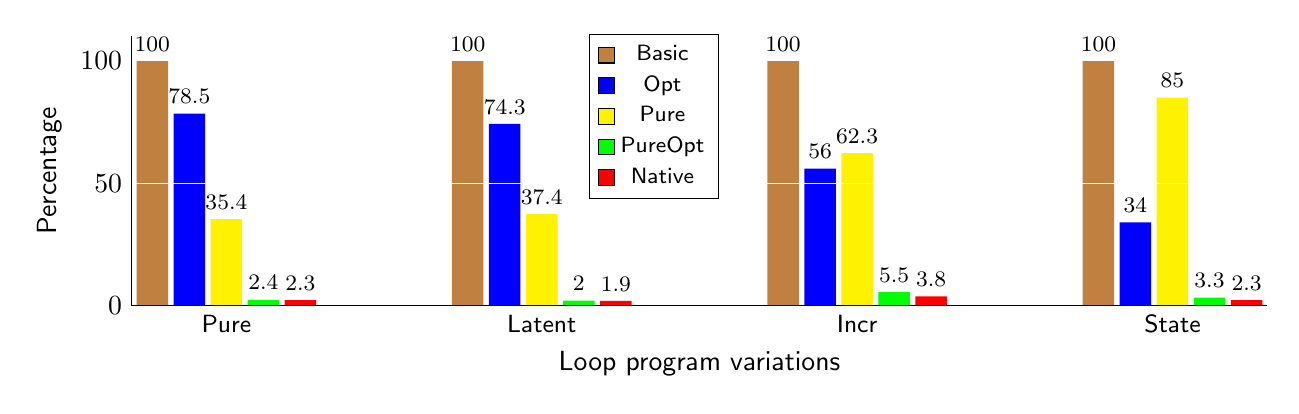
\begin{tikzpicture}
  \centering
  \begin{axis}[
        ybar, axis on top,
        height=5cm, width=16cm,
        ymajorgrids, tick align=inside,
        bar width=0.4cm,
        major grid style={draw=white},
        enlarge y limits={value=.1,upper},
        ymin=0, ymax=100,
        axis x line*=bottom,
        axis y line*=left,
        y axis line style={opacity=1},
        tickwidth=0pt,
        xtick = data,
        x tick label style={font=\small,text width=1.4cm,align=center},
         enlarge x limits=true,
      legend image code/.code={%
      \draw[#1] (0cm,-0.1cm) rectangle (0.2cm,0.1cm);
    },
            legend style={
            at={(0.46,1.01)},
            anchor=north,
            % legend columns=-1,
            % /tikz/every even column/.append style={column sep=0.4cm},
            font = \footnotesize
        },
        ylabel={Percentage},
        xlabel={Loop program variations},
           symbolic x coords={
           Pure,
           Latent,
           Incr,
           State,
           },
            nodes near coords={
         \footnotesize \pgfmathprintnumber{\pgfplotspointmeta}
        }
    ]
   \addplot [draw=none,fill=brown] coordinates {
      (Pure,100)
      (Latent,100)
      (Incr,100)
      (State,100)
       };

    \addplot [draw=none,fill=blue] coordinates {
      (Pure,78.5)
      (Latent,74.3)
      (Incr,56)
      (State,34)
      };

    \addplot [draw=none,fill=yellow] coordinates {
      (Pure,35.4)
      (Latent,37.4)
      (Incr,62.3)
      (State,85)
       };

    \addplot [draw=none,fill=green] coordinates {
      (Pure,2.4)
      (Latent,2)
      (Incr,5.5)
      (State,3.3)
       };

    \addplot [draw=none,fill=red] coordinates {
      (Pure,2.3)
      (Latent,1.9)
      (Incr,3.8)
      (State,2.3)
       }; 
   

    \legend{Basic, Opt, Pure, PureOpt, Native}
  \end{axis}
  \end{tikzpicture}
\caption{Relative run-times of Loops example  \cite{own}}
\label{fig:loops}
\end{figure}

\begin{figure}[H]
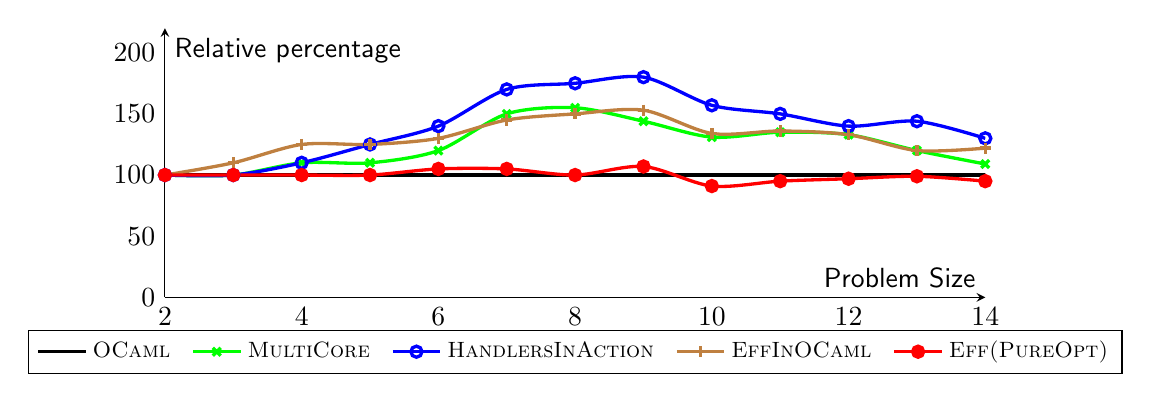
\begin{tikzpicture}
  \centering
  \begin{axis}[
        axis lines=center,
        axis on top,
        height=5cm, width=12cm,
        % bar width=0.4cm,
        % ymajorgrids, tick align=inside,
        major grid style={draw=white},
        enlarge y limits={value=.1,upper},
        ymin=0, ymax=200,
        axis x line*=bottom,
        axis y line*=left,
        % xtick = data,
        y axis line style={opacity=1},
        tickwidth=0pt,
        enlarge x limits=false,
        legend style={
            at={(0.5,-0.12)},
            anchor=north,
            legend columns=-1,
            /tikz/every even column/.append style={column sep=0.2cm},
            font = \footnotesize
        },
        ylabel={Relative percentage},
        xlabel={Problem Size},
           % symbolic x coords={
           % 0,
           % 8,
           % 9,
           % 10,
           % 11,
           % 12,
           % % 13,
           % % 14
           % },
       %      nodes near coords={
       %  \pgfmathprintnumber{\pgfplotspointmeta}
       % }
    ]
    %native
    \addplot [smooth,color = black, very thick] coordinates {
      (2,100)
      (3,100)
      (4,100)
      (5,100)
      (6,100)
      (7,100)
      (8,100)
      (9,100)
      (10,100)
      (11,100)
      (12,100)
      (13,100)
      (14,100)
       };
    %multicore
    \addplot [smooth,color = green, very thick, mark = x] coordinates {
      (2,100)
      (3,100)
      (4,110)
      (5,110)
      (6,120)
      (7,150)
      (8,155)
      (9,144)
      (10,131)
      (11,135)
      (12,133)
      (13,120)
      (14,109)
       };
    %HIA
   \addplot [smooth,color = blue, very thick, mark = o] coordinates {
      (2,100)
      (3,100)
      (4,110)
      (5,125)
      (6,140)
      (7,170)
      (8,175)
      (9,180)
      (10,157)
      (11,150)
      (12,140)
      (13,144)
      (14,130)
       };
    %EffectsinOcaml
   \addplot [smooth,color = brown, very thick, mark = +] coordinates {
      (2,100)
      (3,110)
      (4,125)
      (5,125)
      (6,130)
      (7,145)
      (8,150)
      (9,153)
      (10,134)
      (11,136)
      (12,133)
      (13,120)
      (14,122)
       };
    %PureOpt
   \addplot [smooth,color = red, very thick, mark = *] coordinates {
      (2,100)
      (3,100)
      (4,100)
      (5,100)
      (6,105)
      (7,105)
      (8,100)
      (9,107)
      (10,91)
      (11,95)
      (12,97)
      (13,99)
      (14,95)
       };

    \legend{\ocaml, \textsc{MultiCore}, \textsc{HandlersInAction}, \textsc{EffIn\ocaml}, \textsc{\eff}\textsc{(PureOpt)}}
  \end{axis}
  \end{tikzpicture}
\caption{Results of running N-Queens for all solutions on multiple systems  \cite{own}}
\label{fig:systemsall}
\end{figure}
\begin{figure}[H]
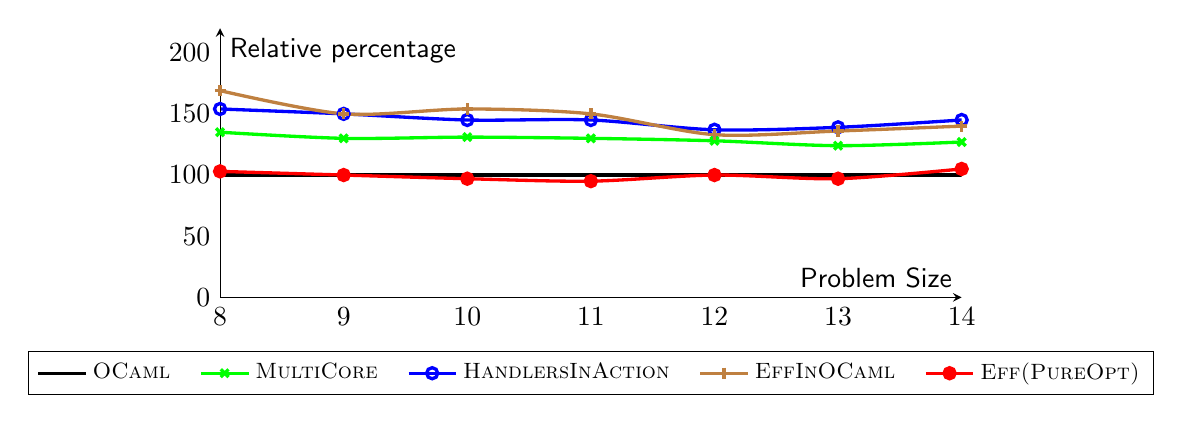
\begin{tikzpicture}
  \centering
  \begin{axis}[
        axis lines=center,
        axis on top,
        height=5cm, width=11cm,
        % bar width=0.4cm,
        % ymajorgrids, tick align=inside,
        major grid style={draw=white},
        enlarge y limits={value=.1,upper},
        ymin=0, ymax=200,
        axis x line*=bottom,
        axis y line*=left,
        xtick = data,
        y axis line style={opacity=1},
        tickwidth=0pt,
        enlarge x limits=false,
        legend style={
            at={(0.5,-0.2)},
            anchor=north,
            legend columns=-1,
            /tikz/every even column/.append style={column sep=0.3cm},
            font = \footnotesize
        },
        ylabel={Relative percentage},
        xlabel={Problem Size},
           % symbolic x coords={
           % 0,
           % 8,
           % 9,
           % 10,
           % 11,
           % 12,
           % % 13,
           % % 14
           % },
       %      nodes near coords={
       %  \pgfmathprintnumber{\pgfplotspointmeta}
       % }
    ]
    %native
    \addplot [smooth,color = black, very thick] coordinates {
      % (0,100)
      (8,100)
      (9,100)
      (10,100)
      (11,100)
      (12,100)
      (13,100)
      (14,100)
       };
    %multicore
    \addplot [smooth,color = green, very thick, mark = x] coordinates {
      (8,135)
      (9,130)
      (10,131)
      (11,130)
      (12,128)
      (13,124)
      (14,127)
       };
    %HIA
   \addplot [smooth,color = blue, very thick, mark = o] coordinates {
      (8,154)
      (9,150)
      (10,145)
      (11,145)
      (12,137)
      (13,139)
      (14,145)
       };
    %EffectsinOcaml
   \addplot [smooth,color = brown, very thick, mark = +] coordinates {
      (8,169)
      (9,150)
      (10,154)
      (11,150)
      (12,133)
      (13,136)
      (14,140)
       };
    %PureOpt
   \addplot [smooth,color = red, very thick, mark = *] coordinates {
      (8,103)
      (9,100)
      (10,97)
      (11,95)
      (12,100)
      (13,97)
      (14,105)
       };

    \legend{\ocaml, \textsc{MultiCore}, \textsc{HandlersInAction}, \textsc{EffInOCaml}, \textsc{\eff}\textsc{(PureOpt)}}
  \end{axis}
  \end{tikzpicture}
\caption{Results of running N-Queens for one solution on multiple systems  \cite{own}}
\label{fig:systemsone}
\end{figure}



\section{Reflection}
\subsection{General reflection}
An important, if not the most important, aspect that I learned, is that there is no shame in asking for help. This is a competency I didn't think I would learn, it is also not a competency I thought was a problem. More specifically, during the honoursproject I realised that it was better to ask a lot of questions and timely tell someone when I'm having issues then to wait. \\
\\
In the proposal, I said that the honoursprogramme provided an excellent opportunity to get involved with research. Looking back, this has become the most important reason for me. Without the honoursprogramme, I would have a different view of what research is like. I also said that I liked the challenge. In the end, the honoursproject was even more challenging than I expected it to be. Instead of doing the honoursprogramme over a period of the entire academic year, I completed it in nearly one semester. Because I really enjoyed the challenge that the honoursprogramme provided me, I decided to take the second honoursproject this year aswell. This means that I will complete the entire honoursprogramme in a single year.

\subsection{Relation between honoursprogramme and degree}
The honoursproject is linked to my master degree. The honoursproject helped me decide what I want to do for my masterthesis. My second honoursproject goes further in the effect handlers project. Both honoursprojects build up towards my masterthesis. This is an interesting result from doing the honoursprojects within the computer science departement. If I didn't do my honoursproject within the computer science departement, I wouldn't be able to use the honourprojects as a build up for the masterthesis. This is also something that wasn't planned in advance.  \\
\\
During my bachelors, I had a course on functional and logical programming. This course was useful since it provided me with knowledge about the functional programming paradigm. Though it wasn't a course, I have done several research internships. The content of these internships were not related to programming languages. However, these internships did prepare me for the honoursproject. It taught me how to work independently. \\
\\
There is also a course on Formal Systems and their Applications (H04H8BE) which revolves around the typical structure and composition of a formal system such as the lambda calculus. It is taught during the second semester. I was planning to take this course at first, since the content seemed relevant to my honoursproject. However, since my honoursproject occured throughout the first semester, I wasn't able to take the course and possibly take advantage of the content. \\
\\
Other than these courses, there weren't any courses which directly link to the honoursproject. However there was a synergy between the honoursproject and the courses I followed. This synergy came from the fact that my specialisation, Artificial Intelligence, is linked to the research group where I'm doing my honoursproject.

\subsection{Workload of the honoursprogramme}
In the proposal of the honoursproject, it was also discussed that doing the entire honoursprogramme during the masters would be difficult. To make my second year more bearable, I chose to spend 70 ECTS credits on courses during my first year instead of the usual 60 ECTS credits. This has to consequence that my first year would be even more difficult compared to the honoursproject added to the usual 60 ECTS credits. \\
\\
My academic year hasn't ended yet, but I can say that it wasn't a mistake to take the 70 ECTS credits. It was a huge workload, but it also had another unintended effect. My time management skills improved significantly. The fact that I'm also taking my second honoursproject this year tells that I'm motivated and able to handle the workload. \\
\\
In general, I found the workload of the honoursprogramme to be comparable to the workload of 9 ECTS credits. 

\subsection{Social relevance}
In the initial proposal, it was said that the honoursproject is socially relevant for multiple reasons. Society continuously demands more, faster and more reliable software. If better tools for programming languages are developed, this demand can be satisfied faster. A type-\&-effect system makes it easier to implement backtracking, non-determinism and more. It also makes it easier to detect bugs within a program. Optimizing a type-\&-effect system makes it more viable to use such a system in commercial software. 


\section{Conclusions}
\subsection{Looking back}
I was able to accomplish more than I expected in the honoursproject. I expected that I could only implement one optimization and that by then I would be done. Multiple optimizations were implemented. In this regard, I underestimated the amount of work I could do in the honoursproject. \\
\\
However, It took longer to orientate myself in the landscape of algebraic effect handlers than I expected. I found that there is a big difference between getting familiar enough with algebraic effects and handlers so I could use them within programs and getting familiar enough with algebraic effects and handlers so I could do research within that field. More specifically, I could write small programs that use algebraic effects and handlers quite fast, but it took a lot longer to be able to do the optimizations. 

\subsection{Where the goals reached}
In the motivation letter, multiple steps were given that needed to be accomplished.
\begin{enumerate}
\item Literature study of Eff and existing optimizations \label{literature}
\item Designing new optimizations \label{design}
\item implementation \label{implementation}
\item evaluation through benchmarks \label{evaluation}
\item formal proof of the optimizations \label{proof}
\end{enumerate}
These steps, with the exclusion of step~\ref{proof}, were accomplished. In the group, it was decided that it was best for me to continue working on the benchmarks and writing the paper instead of writing formal proofs. \\
\\
Step~\ref{literature} was the first task that was accomplished. This was essential for me to be able to contribute to the research project. Afterwards step~\ref{design} and step~\ref{implementation} were done in parallel. Finally step~\ref{evaluation} and working on the paper were done. 

\subsection{Value of the Honoursprogramme}
Other goals that are important for the honoursprogramme concern my own contributions and the knowledge and experience that were gained. During the honoursproject, I was partly treated as an honoursstudent and partly as a researcher. I was partly treated as an honourstudent since I did have regular meetings with professor Schrijvers. But I was also treated as a researcher as I did have a voice during meetings for the project. This meant that I was able to make contributions and state my opinion about decisions before they are made. Ofcourse this came with the responsibility that I carried my own weight.\\
\\
I would say there were a lot of values to the honoursproject. Some I have already mentioned. I got introduced to being a researcher. The honoursproject was quite a challenge, which I definitely found a value of the honoursproject.  I believe that because of these values, my thirst for more knowledge also increased. I want to delve deeper into type-\&-effect systems, learn more about the theoretical foundations. 

\subsection{Conclusion}
To conclude, something that definitely needs to be said is that I'm proud of what I've accomplished during this honoursproject. Choosing to participate in the honoursprogramme and doing my honoursproject with professor Schrijvers were the best choices I could have made. The honoursproject taught me a lot about research, programming language theory and myself. 


\appendix
\section{Competencies}
\textbf{Theoretical and mathematical foundations of computer science}: I wanted to expand my knowledge of the theoretical and mathematical foundations of computer science. I found that I have improved this competency. More specifically, I learned about algebraic effect handlers and formal type systems. However, my thirst for more knowledge has only increased since starting the honoursproject. I want to learn more about type systems and algebraic effect handlers, especially about the theoretical foundations. \\
\\
\textbf{Oral communication}: I learned a lot about this competency. I was able to discuss decisions to be made in the project with other researchers. In the weekly meetings, each researcher had to talk about the progress made and the issues encountered during the previous week. I feel like I was more shy towards the beginning of the honoursproject. This has gotten a lot better during the honoursproject. However, I feel like I cannot always express my thoughts in the correct scientific terms. That is definitly a working point for the future. Most communication happened in English. It was really interesting and fun to communicate professionally in English. I didn't think that improving my English communication skills was a competency I was going to learn. However, my communication skills did improve during the honoursproject. A skill that I wanted to improve was given presentations for a larger audience. However, this is something that does not really occur during the honoursproject. \\
\\
\textbf{Written communication}: I improved this competency less than I expected. It also improved in a different way than I expected. I expected to improve my competency in writing reports. However, I didn't write many reports for this honoursproject. I did write portions of the paper, which improved my academic writing competency. This is a competency that still needs to be improved a lot. More specifically, my academic writing skills need to be improved. \\
\\
\textbf{Asking for help}: As explained before, this is one of the most important competencies that I learned. I didn't think I would learn this competency, since I never realised that this was something that needed improvement. In a research project, it is important to understand the material, but there is also a deadline. That means that without asking for help, things are bound to go awry.  This is something I learned during the honoursproject. However, I do think that this is something that can and needs improvement. Sometimes it occurs that people explain a new concept to me, but I don't fully understand it yet. In those circumstances, I would like to ask for more explanations, however I'm not always sure how to ask for help. I also think that sometimes I assume too quickly that I understand something when it would have been better to ask more questions. These are definitely issues that have a high priority for improvement.\\
\\
\textbf{Time management}: In my reflection I explained that I improved my time management skills. I find this to be an important competency to be learned. Due to the huge workload that I took, which wasn't solely due to the honoursproject, I learned how to efficiently manage my time. I do think that there are still many improvements possible. More specifically, I'm not good at estimating how long a task will take me to execute. I often underestimate or overestimate the amount of time required for certain tasks. This happens mostly with tasks that take less than a week to complete.  \\
\\
\textbf{Interdisciplinary interest}: This competency is not directly linked to my honoursproject, but is more a consequence of the honoursprogramme. Nevertheless, I still find this to be important enough to include in this report. My honoursproject is focused on research and also happens to be within my own discipline. Due to this, the interdisciplinary character of my honoursproject is small.  Due to being part of the honoursprogramme, I also attended intervision moments and honourscommunity meetings. In these meetings I met a lot of new people. Due to these events I learned how different people look towards honoursprogrammes and interdisciplinary work. This is something that broadened my view and is definitely an aspect which I find important. \\
\\
\textbf{Finding my limit}:  As explained above, I improved my time management skills. Another related competency that I improved is how to find my own limits, what I can and cannot do. This is another competency I learned due to the high workload I had. Using the honoursproject I found the bounderies of the amount of work I can do. However, I do think I'm sometimes still overzealous. \\
\\
\textbf{Creating a hypothesis}: This is a competency I wanted to learn. I feel like this is something that improved over the course of the honoursproject. However I still find it difficult to create a hypothesis. An illustration of this is my masterthesis topic. I knew several aspects about my topic. I wanted it to be research related and it should be related to my honoursproject, type systems. However, it was quite difficult to get concrete ideas myself. Partly I believe this comes from not being knowledgeable enough about the field, which is normal since I'm a masterstudent. But partly I also believe that I also need to learn how to look for potential research ideas. 
\section{Term rewriting: code}
\label{code}
Below is the code for the rule rewritting as implemented in the Eff compiler.
\begin{efflisting}[breaklines=true]
  | Handle ({term = Handler h}, c1)
        when (is_pure_for_handler c1 h.effect_clauses) ->
    useFuel st;
    (* Print.debug "Remove handler, since no effects in common with computation"; *)
    reduce_comp st (bind c1 h.value_clause)

  | Handle ({term = Handler h} as handler, {term = Bind (c1, {term = (p1, c2)})})
        when (is_pure_for_handler c1 h.effect_clauses) ->
    useFuel st;
    (* Print.debug "Remove handler of outer Bind, since no effects in common with computation"; *)
    reduce_comp st (bind (reduce_comp st c1) (abstraction p1 (reduce_comp st (handle (refresh_expr handler) c2))))

  | Handle ({term = Handler h}, {term = Bind (c1, {term = (p1, c2)})})
        when (is_pure_for_handler c2 h.effect_clauses) ->
    useFuel st;
    (* Print.debug "Move inner bind into the value case"; *)
    let new_value_clause = optimize_abs st (abstraction p1 (bind (reduce_comp st c2) (refresh_abs h.value_clause))) in
    let hdlr = handler {
      effect_clauses = h.effect_clauses;
      value_clause = refresh_abs new_value_clause;
    } in
    reduce_comp st (handle (refresh_expr hdlr) c1)

  | Handle ({term = Handler h} as h2, {term = Bind (c1, {term = (p, c2)})}) ->
    useFuel st;
    (* Print.debug "Move (dirty) inner bind into the value case"; *)
    let new_value_clause = optimize_abs st (abstraction p (handle (refresh_expr h2) (refresh_comp (reduce_comp st c2) ))) in
    let hdlr = handler {
      effect_clauses = h.effect_clauses;
      value_clause = refresh_abs new_value_clause;
    } in
    reduce_comp st (handle (refresh_expr hdlr) (refresh_comp c1))
    
  | Handle (h, {term = LetRec (defs, co)}) ->
  let handle_h_c = reduce_comp st (handle h co) in
  let res =
    let_rec' defs handle_h_c
  in
  reduce_comp st res
\end{efflisting}

\printbibliography

\end{document}